% Drawing 161-6/01-2 -- folder 161-6, batch 01, archive page 12 (PDF page 13).
% Transcription: à gauche, un cercle sans légende, partagé par des rayons issus d'un point voisin du centre : cinq rayons à peu près également espacés (celui du haut à gauche court et pâle, celui du bas à gauche épais et dépassant le cercle, celui du bas à droite n'atteignant pas le cercle) et un sixième trait, horizontal, vers la gauche ; deux points du bord marqués d'un petit trait, à gauche ; un arc double entre les deux rayons de droite.
% Kind: circle divided by radii (division in five). Method 2 (schematic redraw from the facsimile). Status: ok.
% Notes: A circle drawn as one stroke open at the left (from the top left round by the right and the bottom to the lower left), and the strokes from one inner point, slightly left of and below the centre: towards the top (to the outline), to the right (to the outline), to the lower right (stops short of the outline), to the lower left (heavy and doubled, one of its two strokes overshooting the outline, where a short tick crosses it: the small cross), to the upper left (short and faint, stops well short), and a sixth, horizontal, to the left as far as where the outline would be. At the upper left, where the outline is not drawn, two short strokes (a tick with a bar). Between the right-hand radius and the lower right one, a second arc runs inside the outline. Disagreement in part with the transcription's note (« partagé par cinq rayons »): six strokes leave the centre; five of them are spaced by about 72 degrees, the sixth (horizontal, to the left) is extra. Redrawn 2026-11-10 (issue 128). Question settled by a machine pass on the facsimile, 2026-11-12 (page): six strokes leave the inner point: five about 72 degrees apart and a sixth, horizontal, to the left as far as the outline; the drawing stands. 2026-11-13, Claude Opus 5.5, issue 147, overlay check: not compiled (no TeX in the session); the TikZ was rasterised by a local interpreter and laid over the 236 ppi scan rendered at 400 dpi. Redrawn on the ink: the outline through points moved onto its ink (the fitted ellipse was up to five units off at the bottom), every stroke fitted by least squares on its own ink; each lies on its ink to within about one unit. Changed: the outline is drawn as the page's open stroke, not as an ellipse; the heavy stroke to the lower left is two strokes; the cross at its end is the tick across the longer one; the doubled arc is one inner arc. Not checked by a reader.
% Coordinates: 1 unit = 1 mm = 1/100 of the crop width (bbox in page fractions: [0.13, 0.48, 0.27, 0.58]).
% Redrawn by Claude (claude-fable-5-2), issue #128, 2026-11-10; not checked by a human; not compiled (no TeX in the session); overlay-checked on the scan by Claude Opus 5.5, issue #147, 2026-11-13, not compiled (no TeX in the session).
% Rights: reproduces part of the work -- behind RENDER_TRANSCRIPTS, never published by itself.
\documentclass[tikz,border=3pt]{standalone}
\usepackage{amsmath,amssymb}
\usetikzlibrary{patterns,arrows.meta}
\tikzset{pencil/.style={black!45}, struck/.style={black!35}, mpt/.style={circle,draw,inner sep=1.3pt}, pt/.style={circle,fill,inner sep=0.9pt}, opt/.style={circle,draw,fill=white,inner sep=1.1pt}}
\begin{document}
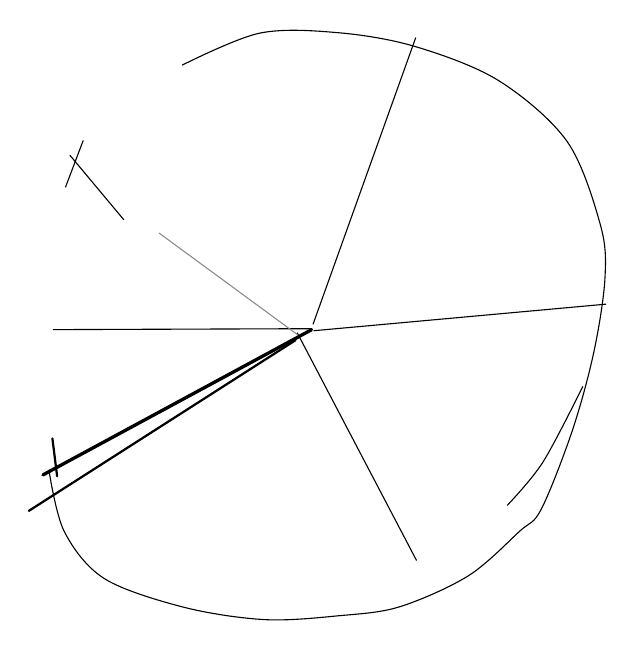
\begin{tikzpicture}[x=1mm,y=1mm,line cap=round,line join=round,font=\scriptsize]
% the outline, open at the left
\draw plot[smooth, tension=0.55] coordinates {(30.2,-21.58) (40.01,-17.53) (49.98,-17.47) (59.75,-19.22) (70.35,-23.54) (79.06,-31.27) (83.27,-41.79) (83.88,-48.55) (82.47,-57.99) (79.74,-67.97) (75.78,-77.99) (73.01,-80.81) (66.53,-86.44) (57.76,-90.39) (50.04,-91.52) (40.68,-92.01) (30.44,-90.45) (20.3,-86.8) (15.2,-80.8) (13.26,-73.02)};
% a second arc inside the outline at the lower right
\draw plot[smooth, tension=0.55] coordinates {(81.05,-62.42) (76,-72) (71.48,-77.48)};
% six strokes from the inner point: five about 72 degrees apart (the one to the lower left heavy and doubled) and a sixth, horizontal, to the left
\draw (46.81,-54.47) -- (59.83,-18.13);
\draw (46.9,-55.32) -- (83.97,-51.95);
\draw (44.8,-55.6) -- (59.93,-84.47);
\draw[very thick] (46.6,-55.2) -- (12.5,-73.63);
\draw[thick] (44.58,-56.52) -- (10.7,-78.2);
\draw[thick] (13.7,-69) -- (14.3,-73.8);
\draw (46.64,-55.06) -- (13.82,-55.18);
\draw[pencil] (44.83,-55.82) -- (27.25,-42.92);
% short strokes at the upper left, where the outline is not drawn
\draw (15.93,-33.04) -- (22.77,-41.23);
\draw (15.37,-37.07) -- (17.6,-31.19);
\end{tikzpicture}
\end{document}
